\section{Implémentation}

\begin{figure}[ht]
  \centering
  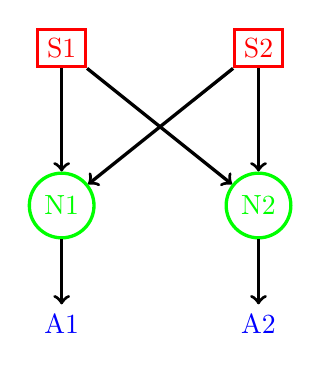
\begin{tikzpicture}[scale=0.5]
 \tikzset{directed/.style={->}} 
  \node[color=blue] (A1) at (0,0) {A1};
  \node[color=blue] (A2) at (5,0) {A2};
  \node[draw, circle, very thick, color=green] (N1) at (0,3) {N1};
  \node[draw, circle, very thick, color=green] (N2) at (5,3) {N2};
  \node[draw, very thick, color=red] (S1) at (0,7) {S1};
  \node[draw, very thick, color=red] (S2) at (5,7) {S2};
  \draw[very thick, directed] (S1) -- (N1);
  \draw[very thick, directed] (S2) -- (N1);
  \draw[very thick, directed] (S1) -- (N2);
  \draw[very thick, directed] (S2) -- (N2);
  \draw[very thick, directed] (N1) -- (A1);
  \draw[very thick, directed] (N2) -- (A2);
\end{tikzpicture}

  \caption{Réseau de neurone à deux neurones}
  \label{graphInit}
\end{figure}

\paragraph{}
Nous pouvons voir sur le schéma \ref{graphInit} que trois types d'objets sont
présents dans notre conception d'un réseau de neurones:\\
\begin{description}
  \item[Les stimuli] Réalisés en rouge sur le schéma, ils génèrent les signaux
    qui activent les premiers neurones et ainsi active le réseau.
  \item[Les actions] Affichés en bleu sur le schéma, elles sont les sorties de
    notre système, elles correspondent à la décision effectué par notre réseau.
  \item[Les neurones] Cœur même du réseau, ils sont là pour effectuer la prise
    de décision en fonction des entrées qu'ils possèdent.
\end{description}

\paragraph{}
Ces trois éléments sont donc la base de notre réseau. Ainsi notre classe correspondant
à un réseau de neurones stocke une liste de stimuli, une liste de réactions et une
liste des neurones constituant le réseau.

\paragraph{}
Il a ensuite fallu déterminer la façon de parcourir tous les neurones pour les
mettre à jour. Cette réflexion a fait émerger deux méthodes. Ces methodes
avaient un impact sur l'implémentation de la classe neurone.\\

\begin{enumerate}
  \item La première consistait, en partant des réactions, à remonter de façon
    récursive le réseau de neurones afin de récupérer les informations pour
    calculer si oui ou non les réactions ont été activées. Cet méthode impliquait
    que chaque neurone ait accès à l'ensemble de ses entrées afin de les
    interroger pour savoir si leurs neurones ont été activés.
  \item La seconde consistait, en partant des stimuli, à propager les informations
    d'activation jusqu'aux réactions. Dans cette méthode quand un neurone a calculé
    si oui ou non il a été activé, il prévient alors l'ensemble de ces sorties de
    son statut. Un neurone recevant une information d'une de ces entrées la
    sauvegarde et si il a reçu l'ensemble des états de ces entrées alors il
    calcule son propre état et le propage de la même manière.
\end{enumerate}

La seconde solution a été choisie car elle semblait plus intuitive dans la
manière de parcourir le réseau (des stimuli vers les réactions). Avec
l'implémentation choisie, on remarque que la validité du réseau est
conditionnée par l'absence de cycles. En effet, s'il existe un cycle il
devient alors impossible de calculer les états des neurones appartenant au
cycle car chaque neurone a besoin des états des autres neurones du cycle.

\paragraph{}
Ne souhaitant pas attribuer aux neurones des caractéristiques qui ne leur étaient
pas nécessaires, nous nous sommes demandé ce qui était intrinsèque au
fonctionnement de l'entité et ce qui relevait de la particularité de notre
réseau. Après réflexion nous sommes arrivé à déterminer comme cœur du neurone, les
parties suivantes:\\

\begin{description}
  \item[Nom]: chaque neurone est doté d'un nom qui permet de le distinguer
    lors de l'envoi de chaque valeur vers les neurones concernés
  \item[Poids]: chaque neurone va pondérer chacune de ses entrées. Ces poids
    sont stockés dans un dictionnaire avec comme clé le nom du neurone et
    comme valeur le poids qui lui est associé.
  \item[Sorties]: la liste des neurones et des réactions connectées à la
    sortie du neurone.
  \item[Inhibiteur]: permet de savoir si le neurone est un inhibiteur ou non.
  \item[Taux d'apprentissage]: le taux de variation des poids du neurone.
\end{description}

\subsection{Fonction d'activation}
Les neurones que nous avons implémentés sont des neurones à seuil,
c'est-à-dire qu'ils accumulent les valeurs des stimuli qu'ils reçoivent et se
déchargent seulement lorsque la somme de ces valeurs dépasse la valeur du
seuil qu'on leur a donné.

Ainsi la fonction d'activation du neurone correspond à la comparaison de la
valeur accumulée avec la valeur du seuil. Lorsque la valeur du seuil est
dépassée, le neurone se décharge et envoie sa valeur de décharge sur toutes
ses sorties.

Il existe deux types de neurones, des neurones excitateurs et des
neurones inhibiteurs. Les neurones excitateurs renvoient 1 lorsqu'ils se
déchargent et les inhibiteurs envoient -1.
Les deux types de neurones renvoient 0 lorsque le seuil n'est pas dépassé.
Cela permet de prévenir leurs sorties de leur mise à jour.

\subsection{Apprentissage}
Lorsque un neurone se décharge, une mise à jour de la valeur de ses poids
d'entrée est effectuée en fonction de la valeur de ces entrées et de sa valeur
de retour. Nous avons implémentées les fonctions de mises à jour suivantes,
en nous inspirant de la méthode de Oja :

$$\Delta w = w_{n+1} - w_{n} = r (x_n - w_n)$$
où $x_n$ est la valeur de l'entrée, $w_n$ est la valeur du poids et
$r$ est le taux d'apprentissage.

Ce calcul est appliqué de manière à renforcer les liens avec des neurones
excitateurs lorsqu'ils envoie une valeur égale à 1 et qu'une sortie est
obtenue et les liens avec les neurones inhibiteurs lorsqu'une valeur de sortie
de 0 est calculée.
